\documentclass[a4paper, titlepage]{article}
\usepackage[T1]{fontenc}
\usepackage[swedish]{babel}
\usepackage[utf8]{inputenc}
\usepackage{graphicx}
\usepackage[normalem]{ulem}
\title{
    Programming Project \\
    C++ Programming(EDA031)
}
\author{
        Department of Computer Science \\
            \\
        Simon Thörnqvist (ada09st1@student.lu.se)
            \and
        Fredrik Pettersson (ada09fpe@student.lu.se)
            \and
        Marcus Lindfeldt (ada08mli@student.lu.se)
            \and
        Daniel Hilton (ael09dhi@student.lu.se)
}
\date{\today}
\begin{document}
\maketitle

\section{Introduction}\label{introduction}
The purpose of this project was to implement a news system similar to the Usenet News. The assignment included the implementation of the server, the client and the communication between them. NNTP was the protocol used for the communication.

The news system contains articles which has a title, an author and text. Articles are created by the users of the system on the client side which are then stored on the server. Each created article is added to a newsgroup.

\section{Requirements}\label{requirements}
We believe that all requirements have been fulfilled.

\section{System Outline}\label{systemoutline}

\subsection{Com}
The package contains the protocol used for communication and the connection class for communication between client and server.

\subsubsection{MessageHandler}
The Message Handler is used to receive and send data via the communication socket. Both the server and the client use this class for sending / receiving commands.

\subsection{Database}

\subsubsection{In Memory}
This implementation of the database stores the information in the primary memory and destroys it when the server is terminated. It simply uses a map to store the newsgroups where the key is the id number of the newsgroup. Each newsgroup has it's own map to store their articles and the key is the id number of the article. Articles store the title, author and text as strings.

\subsubsection{File}
The file-system database stores the information permanently on disk with the use of simple text files and directories. A base directory is chosen and in it each newsgroup is represented by a directory with a name consisting of the newsgroup ID concatenated with the newsgroup name. Each newsgroup directory can have multiple files representing articles. An article file is named by it's ID and the contents consists of the title, author \& article text, each separated by a newline.

\subsection{Server}
 The server listens to a port, waiting for connections. When a conenction has been established it uses Message Interpreter and to intepret commands sent from the client. MessageHandler is used to receive and send data between the client and server. MessageHandler is used to receive and send data between the client and server.   

\subsubsection{Message Interpreter}
The protocol codes sent to the client are read in MessageIntepreter via the Message Handler. Depending on what code was sent different functions are called. When a code matches a code in the protocol a function is called, which calls a function in the database. The database returns a result and Message Interpreter inteprets the result and sends codes back to the client.

\subsubsection{Server Handler}
ServerHandler is the main class on the application server side. It uses the provided server class and utilizes the waitForActivity function to establish a connection with the client. When a connection has been established ServerHandler calls the MessageInterpreter function interpretAndPerform which reads the command from the client.

\subsection{Client}
The client is implemented as to be as easy and intuitive to use from the command line, the command is entered after a certain, stated, input sequence and is then sent as a string to the commandhandler class. The command handler class then parses the input excecutes the corresponding command. The actual implementation of the client-side is designed so that all of the major changes or alterations can be done from the client class. Thus future changes to the implementation of the user interface are all parsed from the client class.

\section{Communication}\label{communication}
An instance of how the data flows in the system is briefly described below.

\begin{enumerate}
    \item The dataflow starts with a client sending a command, this command will be fetched by the waitForActivity() method in the server. This method will return a pointer to that connection.
	\item The server will then try to interpret the command that was sent. This is done by letting a MessageHandler read the data sent on the connection and then interpret what command was sent in the MessageInterpreter.
	\item First a code is read and that determines what type of command was sent. After that the appropriate helper function is called reading the rest of the command according to the protocol. In case of any errors the connection is closed.
	\item When the command is interpreted the correct method is called in the database. Lets say that the client wants to create an article in other words the method createArticle() is called.
	\item First it is verified that the newsgroup exists. If so the article is created with the sent information.
	\item To let the client know that everything went well the server sends back an ACK as described in the protocol.
	\item The server is now once again waiting for an activity on the socket.
\end{enumerate}

\section{Summary}\label{summary}

\newpage
\appendix
\section{UML Diagram}\label{App:AppendixA}
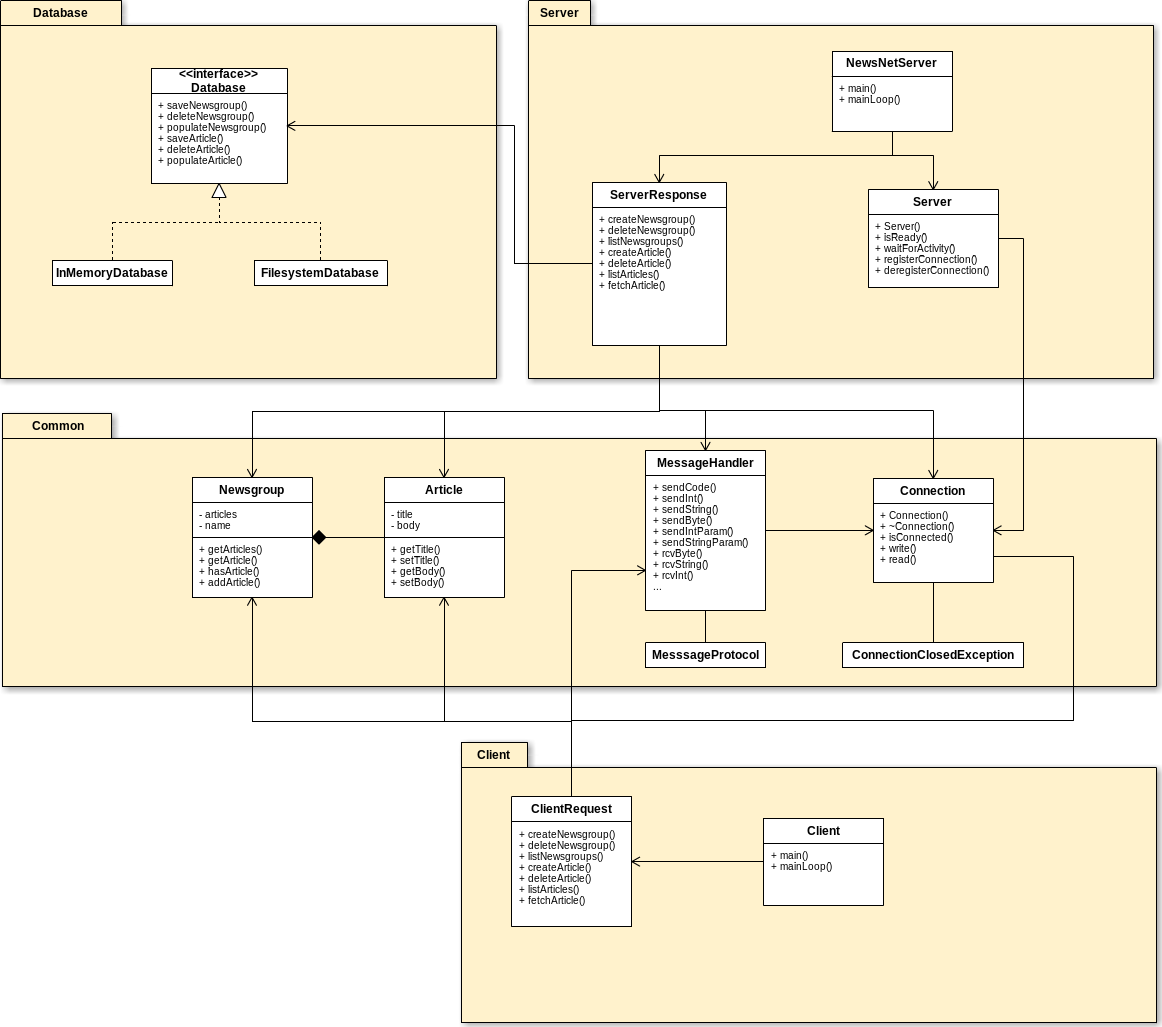
\includegraphics[width=130mm]{NewsNet_UML.png}

\end{document}
